\subsection{W+Jets MC Modelling Validation from CR1}
\label{sec:cr1}


The estimate of the uncertainty on this background is based on CR1, 
defined by applying the full signal selection, including the isolated track veto, but requiring 0 b-tags
(CSV medium working point as described in Sec.~\ref{sec:selection}). 
The sample is dominanted by \wjets\ and is thus used to validate the MC modelling of this background. 

In Table~\ref{tab:cr1mtsf} we show the amount that we need to scale the Wjets MC
by in order to have agreement between data and Monte Carlo in the $M_T$ peak 
region, defined as $60 < M_T < 100$ GeV.  These scale factors are not terribly 
important, but it is reassuring that they are not too different from
1.  [UPDATE WITH TRIGGER EFFICIENCIES]


\begin{table}[!h]
\begin{center}
\begin{tabular}{l||c||c|c|c|c|c}
\hline
Sample              & CR1PRESEL & CR1A & CR1B & CR1C & CR1D & CR1E\\
\hline
\hline
Muon \mt-SF 	  & $0.90 \pm 0.02$ & $0.93 \pm 0.02$ & $0.93 \pm 0.04$ & $0.93 \pm 0.06$ & $1.03 \pm 0.09$ & $1.04 \pm 0.13$ \\
\hline
\hline
Electron \mt-SF 	  & $0.93 \pm 0.02$ & $0.91 \pm 0.03$ & $0.87 \pm 0.05$ & $0.85 \pm 0.07$ & $0.82 \pm 0.09$ & $0.78 \pm 0.13$ \\
\hline
\end{tabular}
\caption{ \mt\ peak Data/MC scale factors applied to the single lepton
  samples and \ttdl. The raw MC is used for backgrounds from rare
  processes. CR1PRESEL refers to a sample with $\met>50$ GeV.
  The uncertainties are statistical only.
\label{tab:cr1mtsf}}
\end{center}
\end{table}


In Table~\ref{tab:cr1yields} we compare the data and MC yields in the four $M_T$ signal regions
and in a looser control region.  We also derive the data/MC scale factors 
$SFR^{e}_{wjet}$ and  $SFR^{\mu}_{wjet}$.  The underlying \met\ and $M_T$ distributions
are shown in Fig.~\ref{fig:cr1met}  and~\ref{fig:cr1mtrest}

\begin{table}[!h]
\begin{center}
{\footnotesize
\begin{tabular}{l||c||c|c|c|c|c}
\hline
Sample              & CR1PRESEL & CR1A & CR1B & CR1C & CR1D & CR1E\\
\hline
\hline
Muon MC 		  & $473 \pm 22$ & $169 \pm 5$ & $116 \pm 4$ & $41 \pm 2$ & $17 \pm 2$ & $8 \pm 1$ \\
Muon Data 		  & $629$ & $238$ & $139$ & $45$ & $12$ & $8$ \\
\hline
Muon Data/MC SF: ($SFR^{\mu}_{wjet}$) 	  & $1.33 \pm 0.08$ & $1.41 \pm 0.10$ & $1.20 \pm 0.11$ & $1.11 \pm 0.18$ & $0.71 \pm 0.21$ & $0.95 \pm 0.36$ \\
\hline
\hline
Electron MC 		  & $327 \pm 8$ & $119 \pm 4$ & $80 \pm 3$ & $30 \pm 2$ & $13 \pm 1$ & $5 \pm 1$ \\
Electron Data 		  & $487$ & $181$ & $103$ & $38$ & $16$ & $6$ \\
\hline
Electron Data/MC SF: ($SFR^e_{wjet}$) 	  & $1.49 \pm 0.08$ & $1.53 \pm 0.13$ & $1.29 \pm 0.14$ & $1.27 \pm 0.22$ & $1.26 \pm 0.35$ & $1.27 \pm 0.56$ \\
\hline
\end{tabular}}
\caption{ Yields in \mt\ tail comparing the MC prediction (after
  applying SFs) to data. CR1PRESEL refers to a sample with $\met>50$
  GeV and $\mt>150$ GeV.
  The uncertainties are statistical only. 
\label{tab:cr1yields}}
\end{center}
\end{table}


\begin{figure}[hbt]
  \begin{center}
        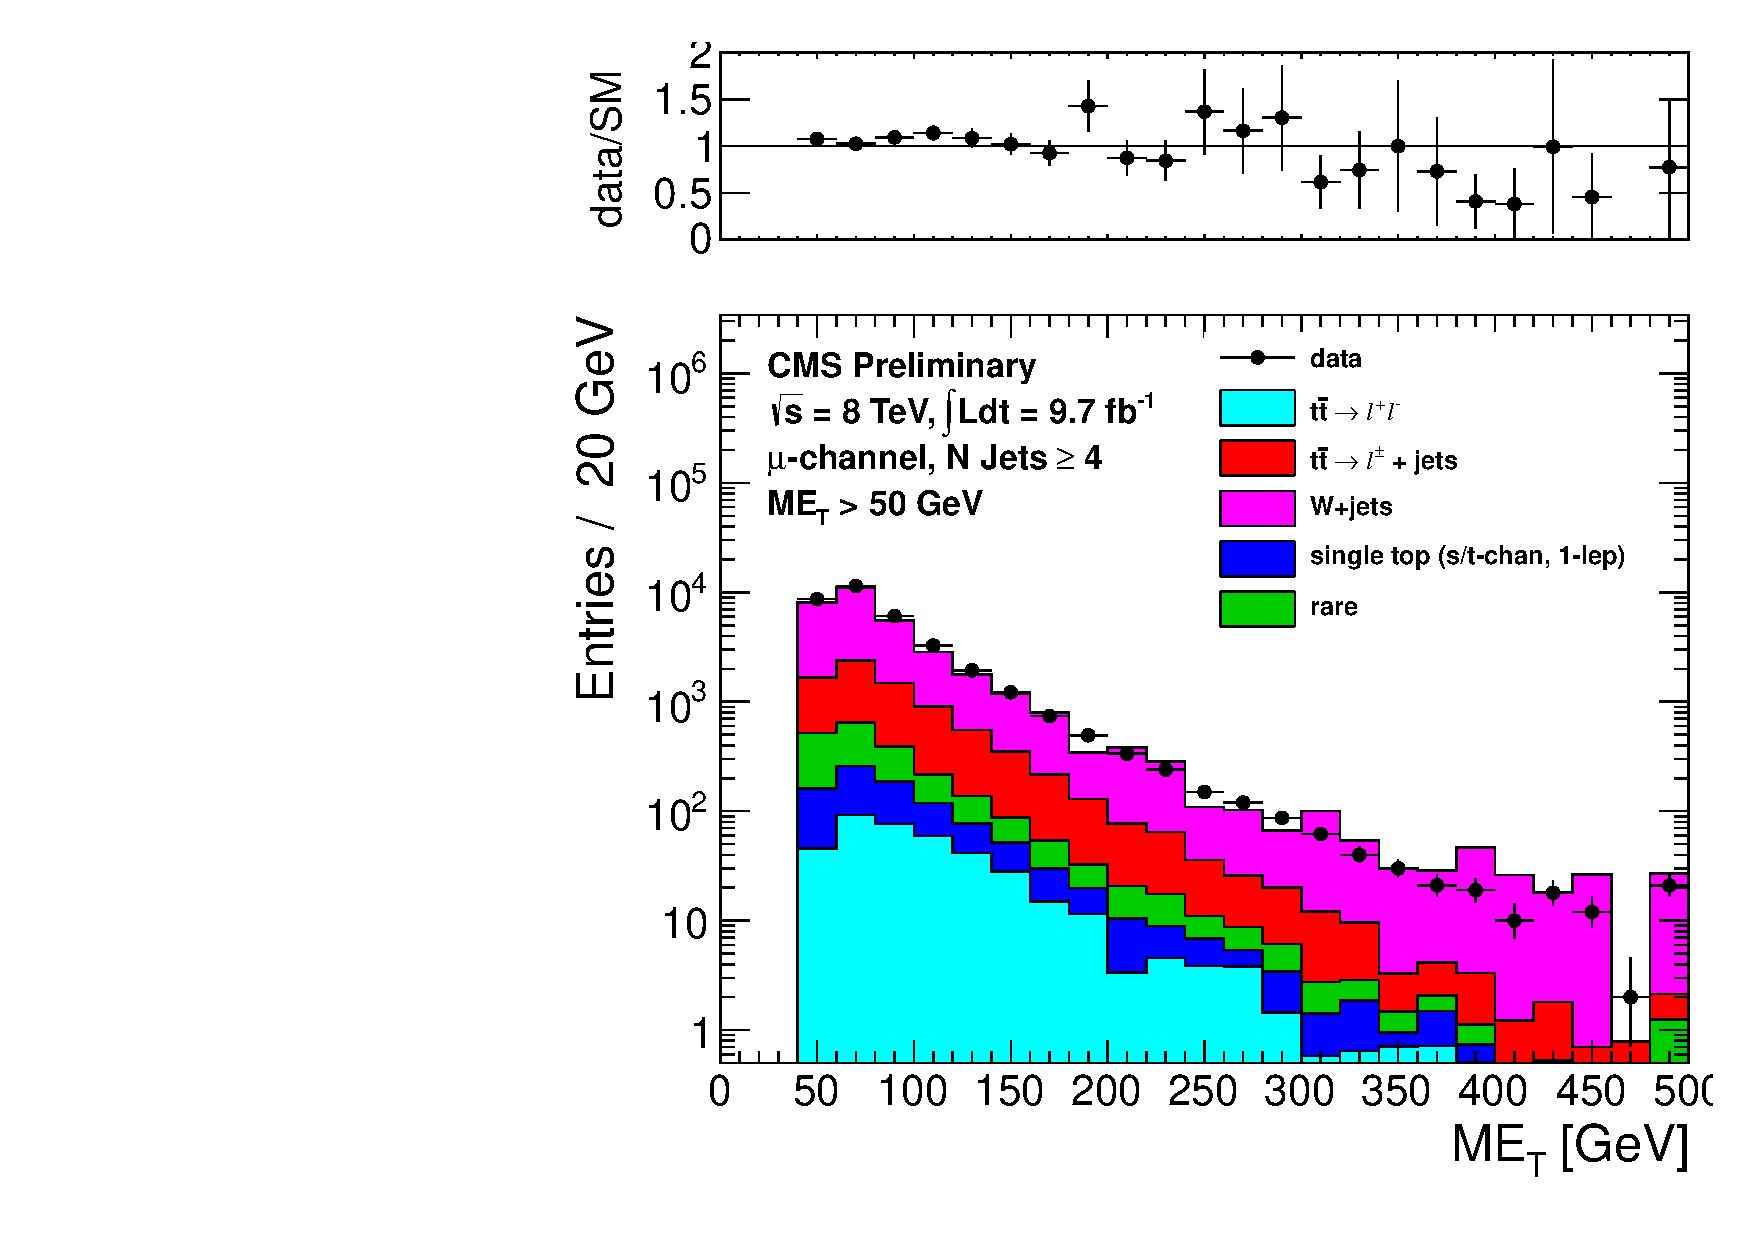
\includegraphics[width=0.5\linewidth]{plots/CR1plots/met_met50_leadmuo_nj4.pdf}%
        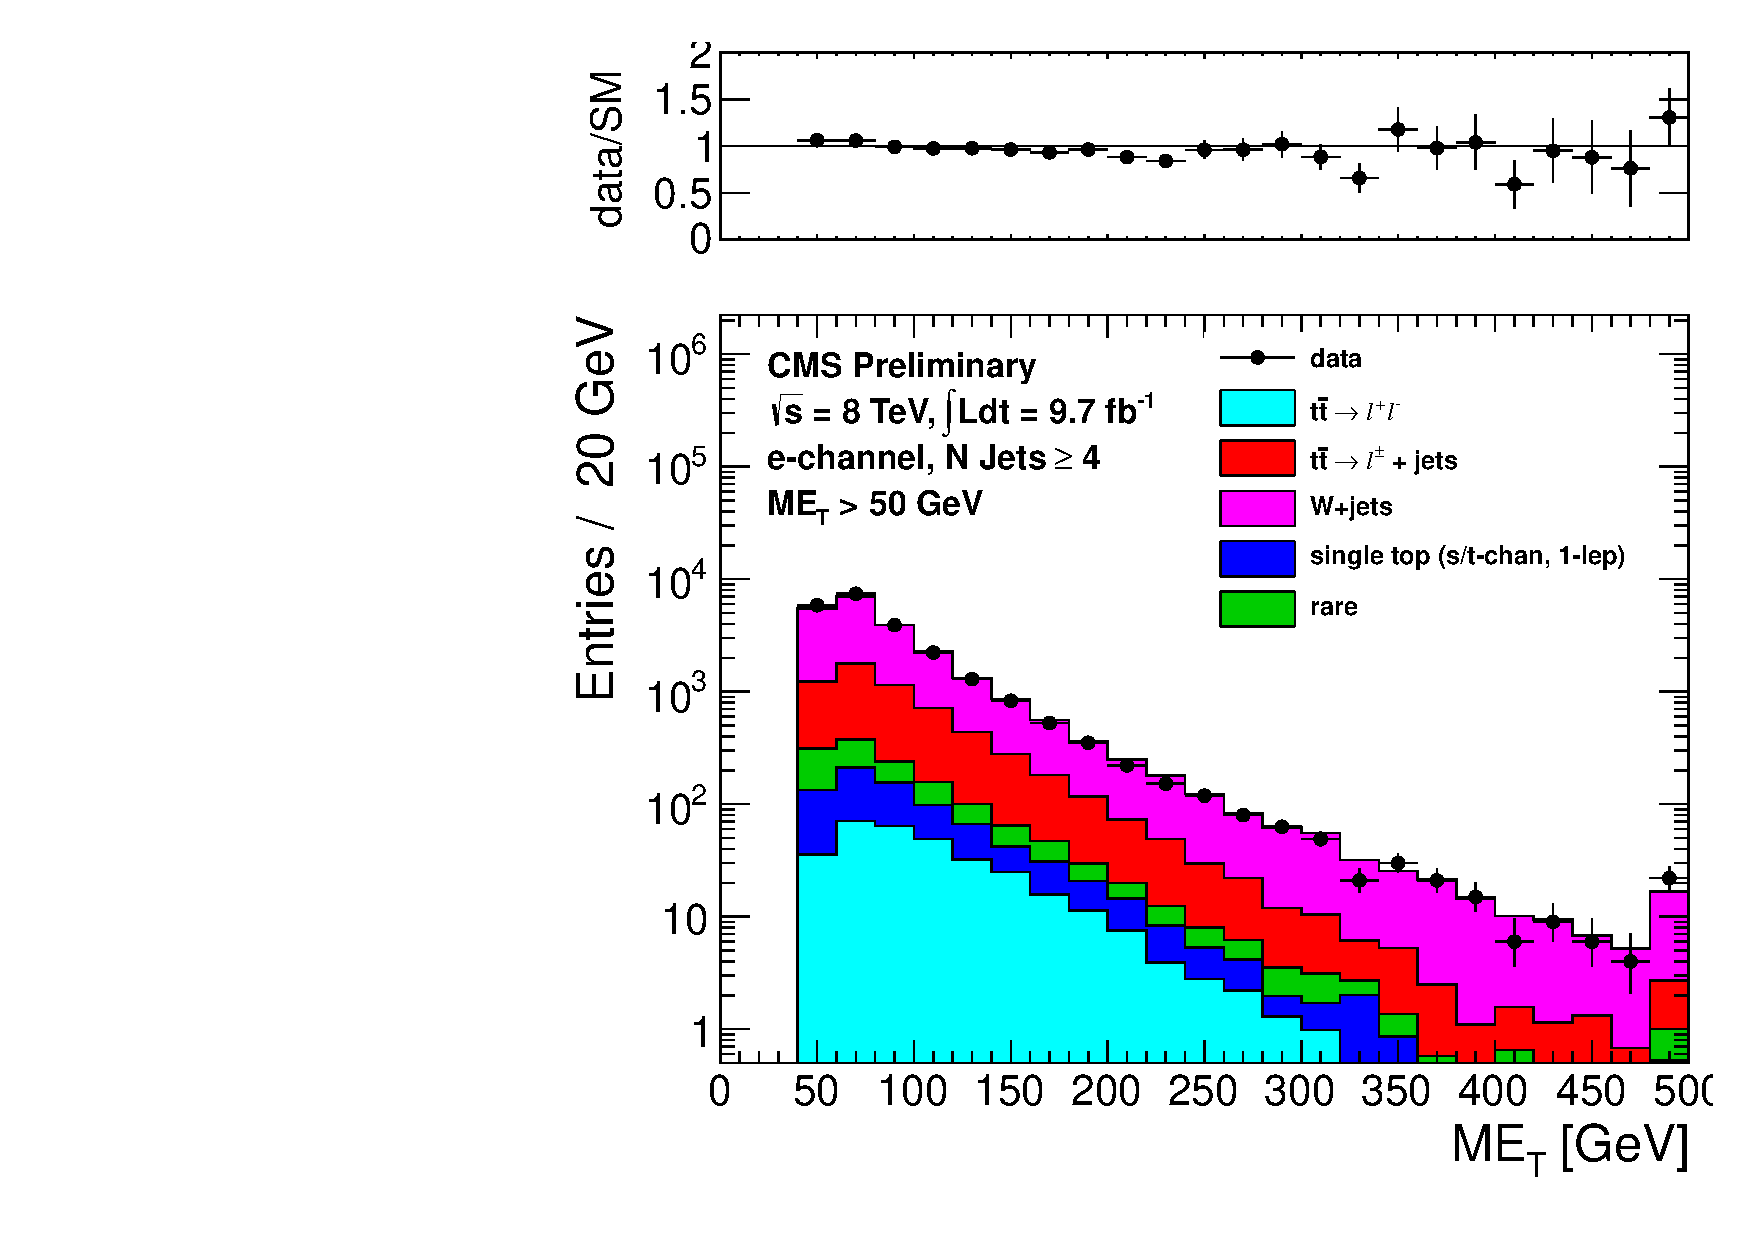
\includegraphics[width=0.5\linewidth]{plots/CR1plots/met_met50_leadele_nj4.pdf}
        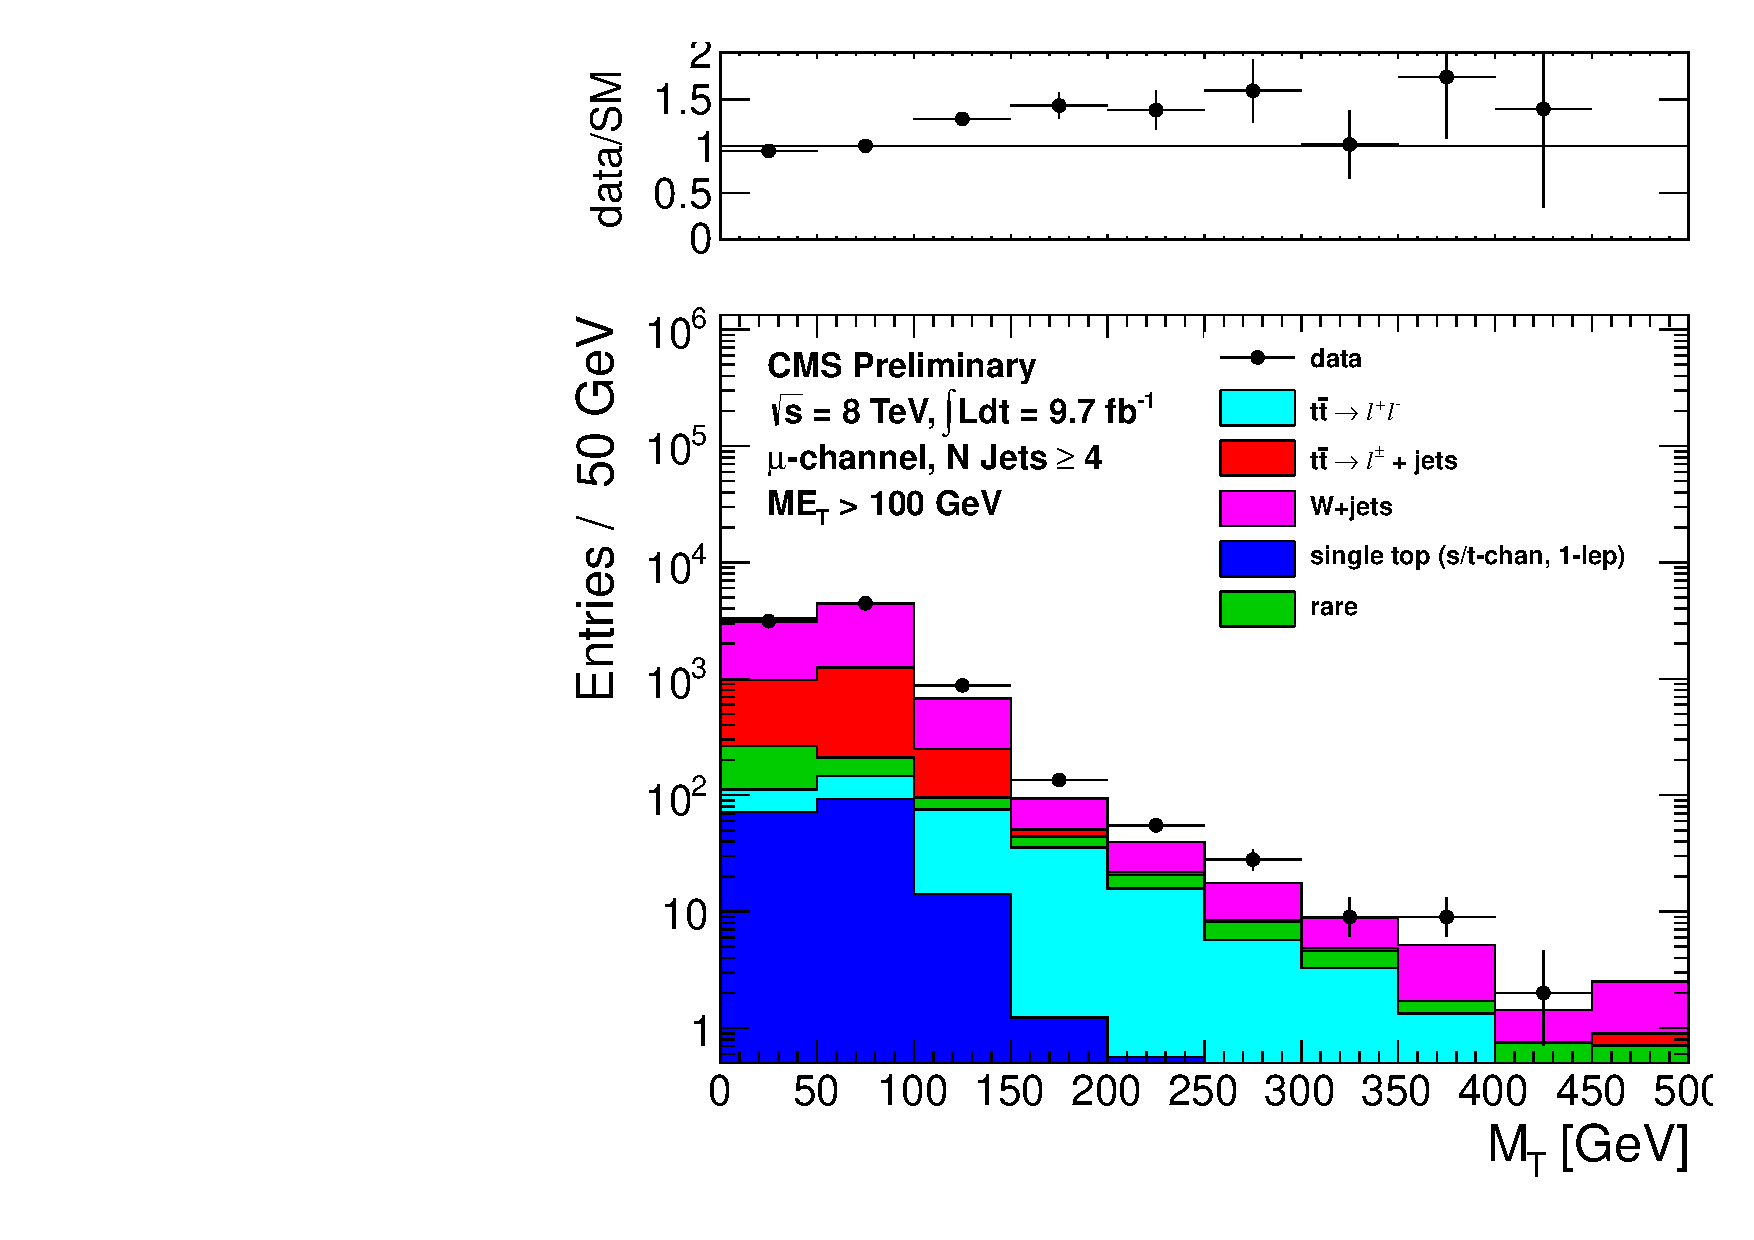
\includegraphics[width=0.5\linewidth]{plots/CR1plots/mt_met100_leadmuo_nj4.pdf}%
        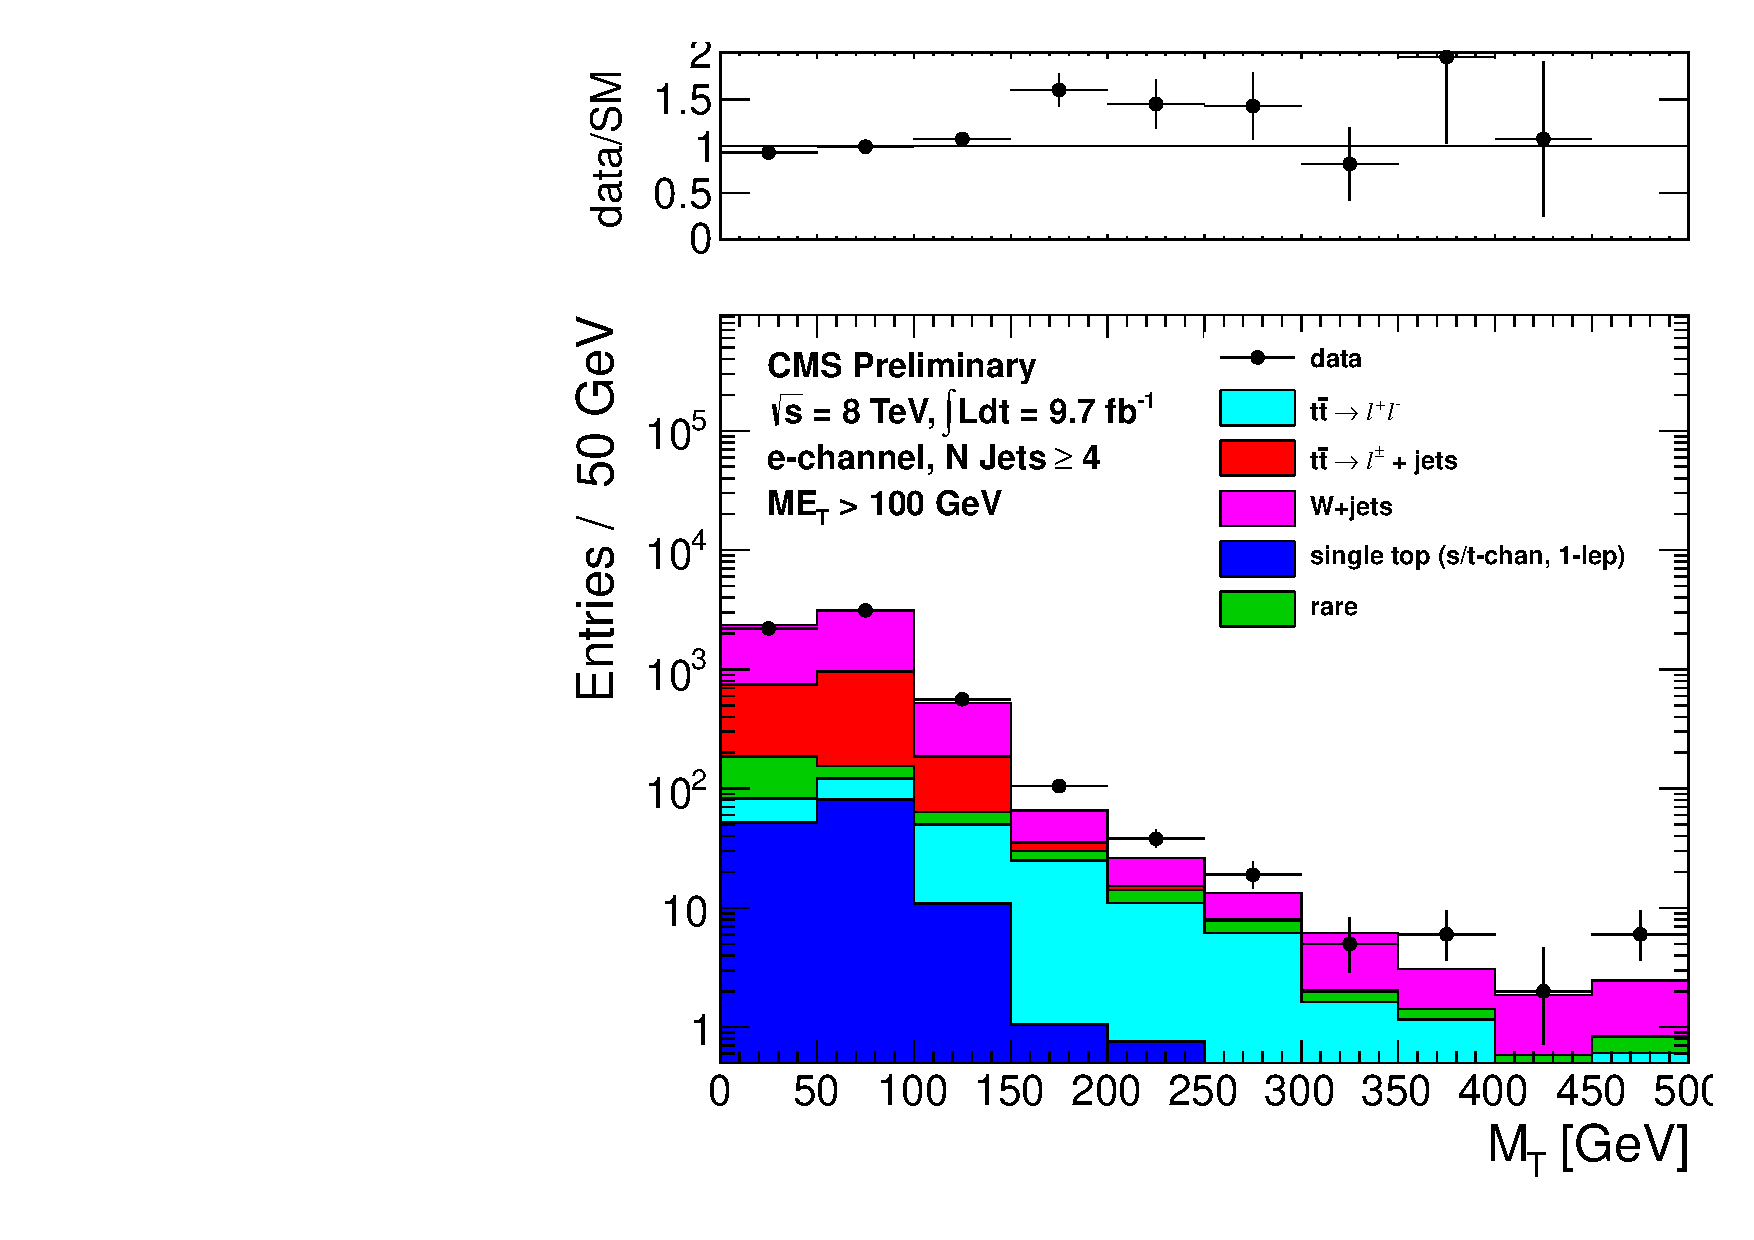
\includegraphics[width=0.5\linewidth]{plots/CR1plots/mt_met100_leadele_nj4.pdf}
    \caption{
      Comparison of the \met\ (top) and \mt\ for $\met>100$ (bottom) distributions in data vs. MC for events
      with a leading muon (left) and leading electron (right)
      satisfying the requirements of CR1. 
\label{fig:cr1met} 
}  
      \end{center}
\end{figure}


\begin{figure}[hbt]
  \begin{center}
        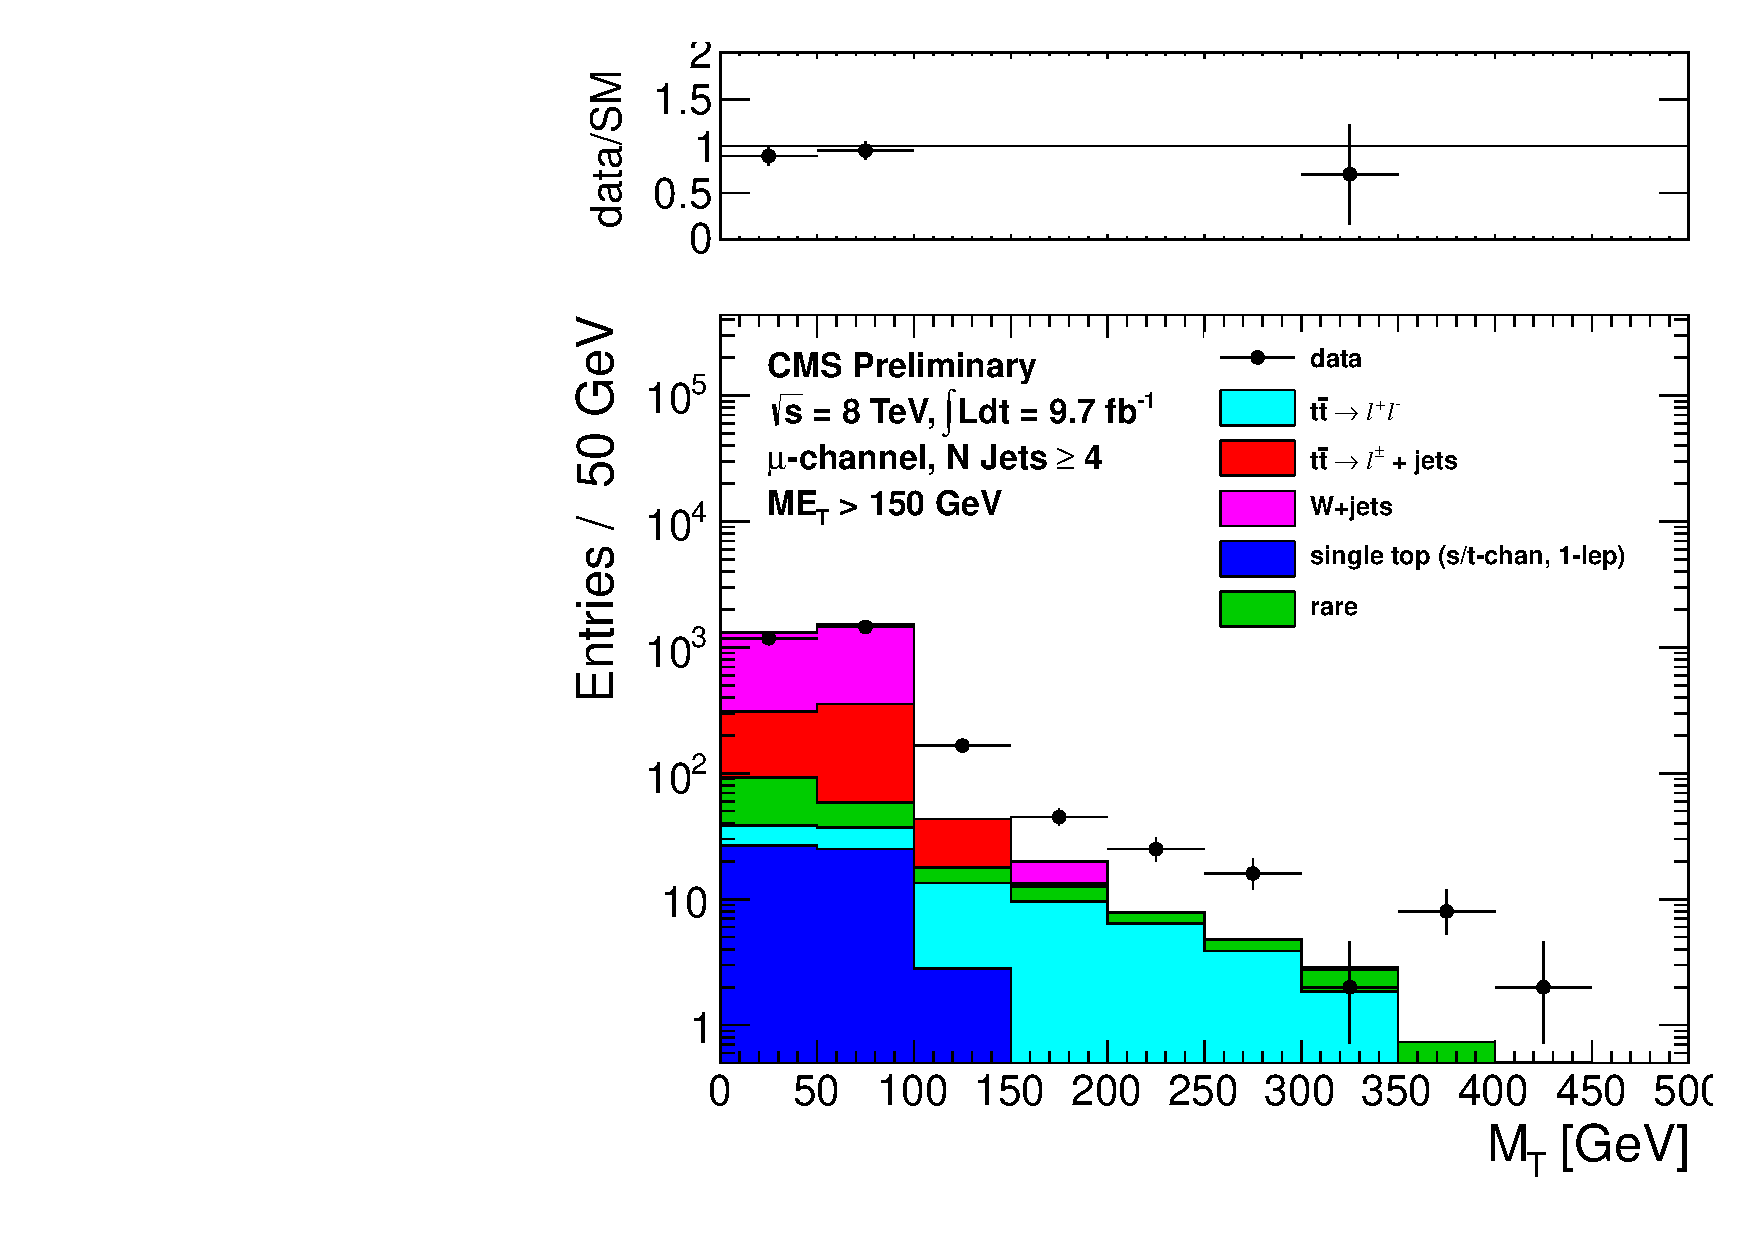
\includegraphics[width=0.5\linewidth]{plots/CR1plots/mt_met150_leadmuo_nj4.pdf}%
        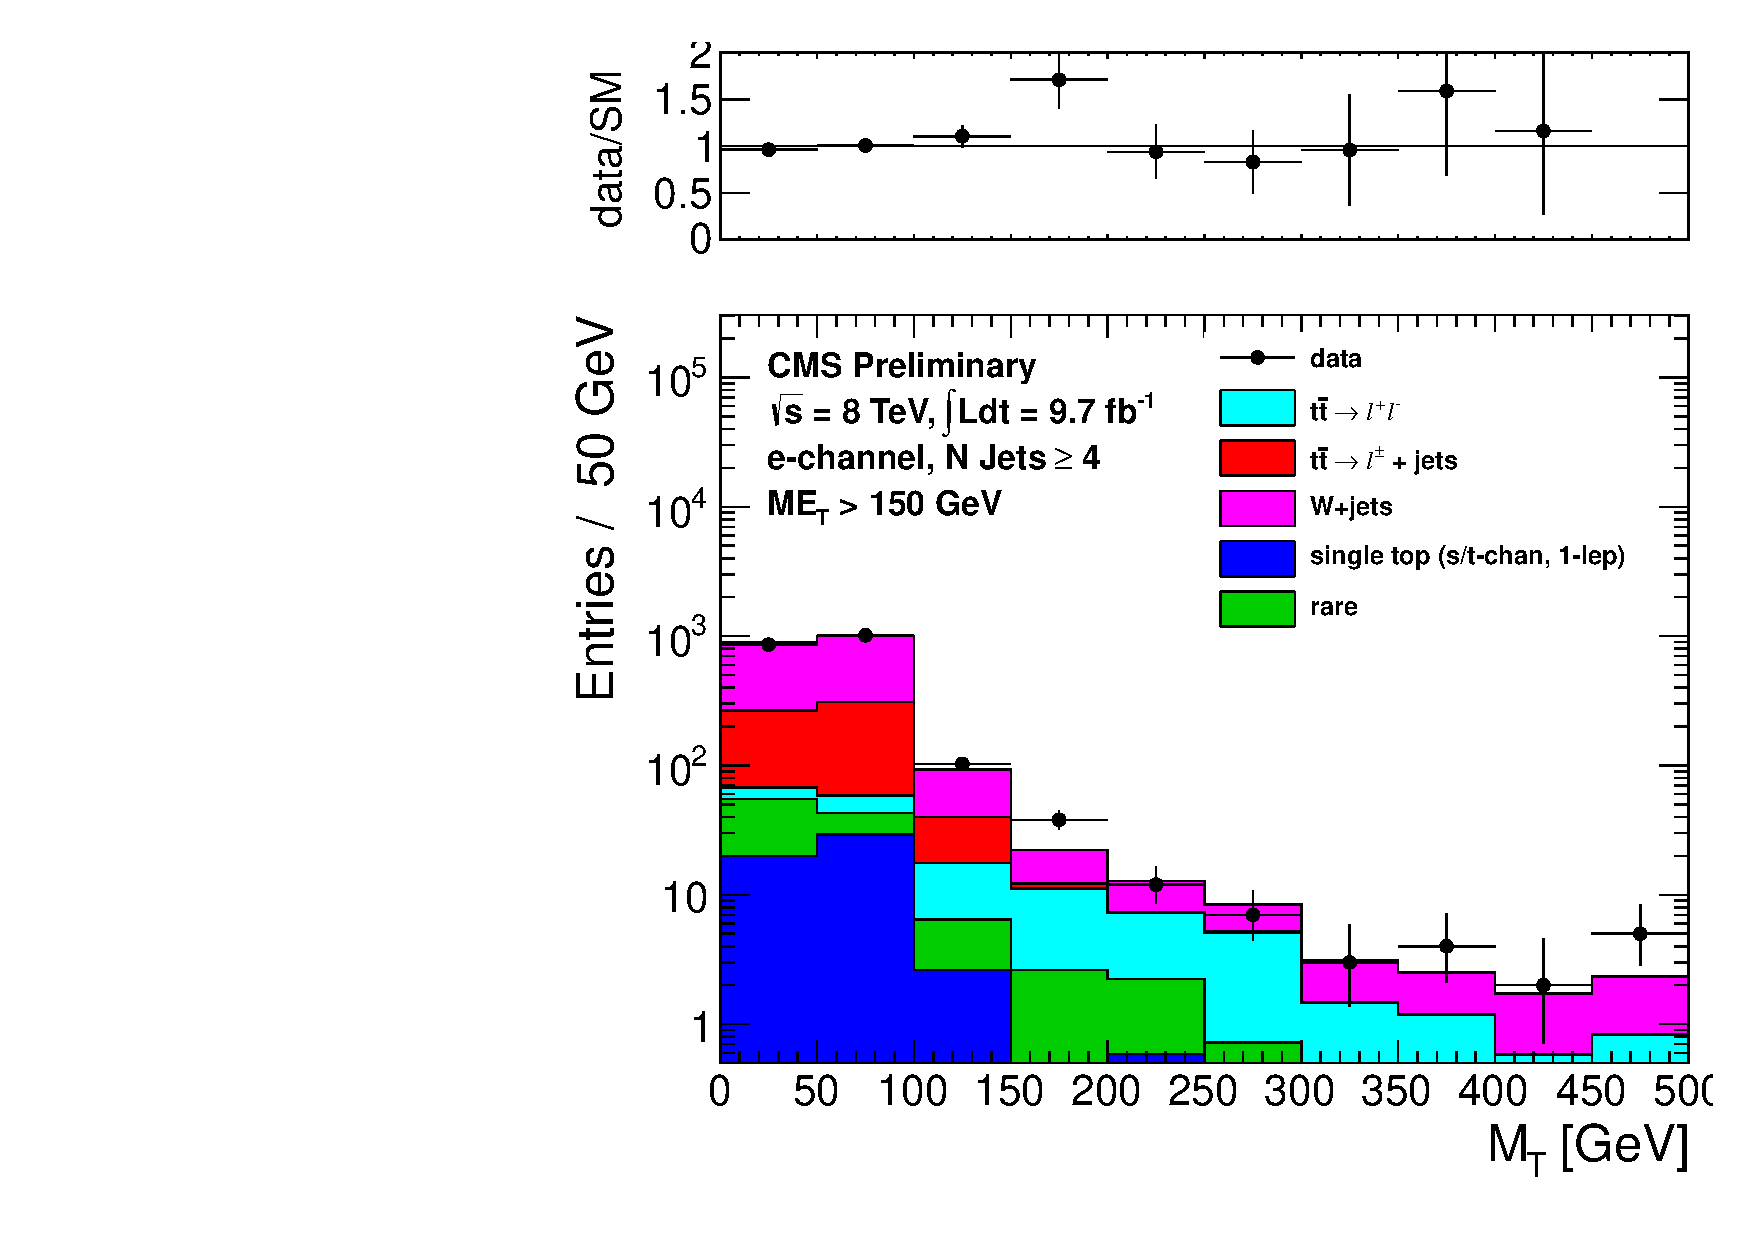
\includegraphics[width=0.5\linewidth]{plots/CR1plots/mt_met150_leadele_nj4.pdf}
        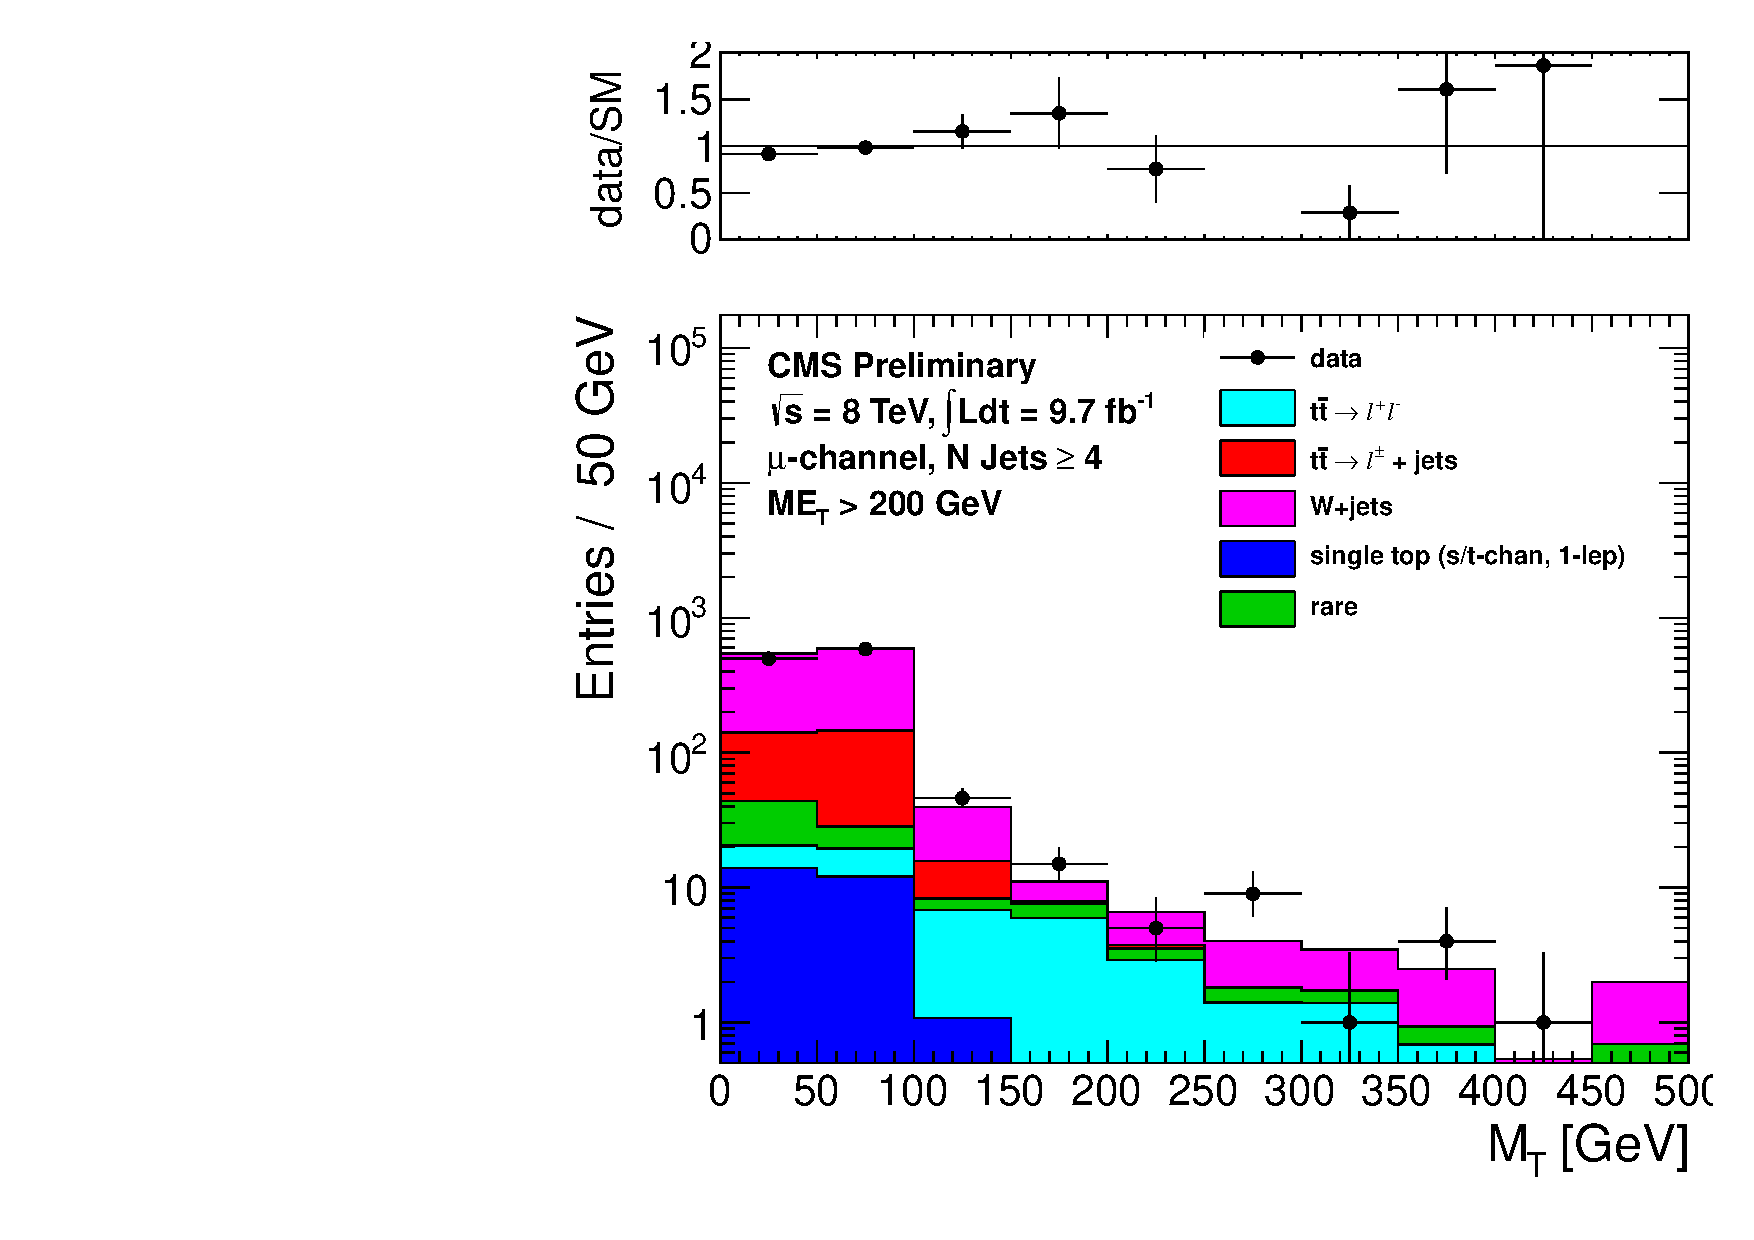
\includegraphics[width=0.5\linewidth]{plots/CR1plots/mt_met200_leadmuo_nj4.pdf}%
        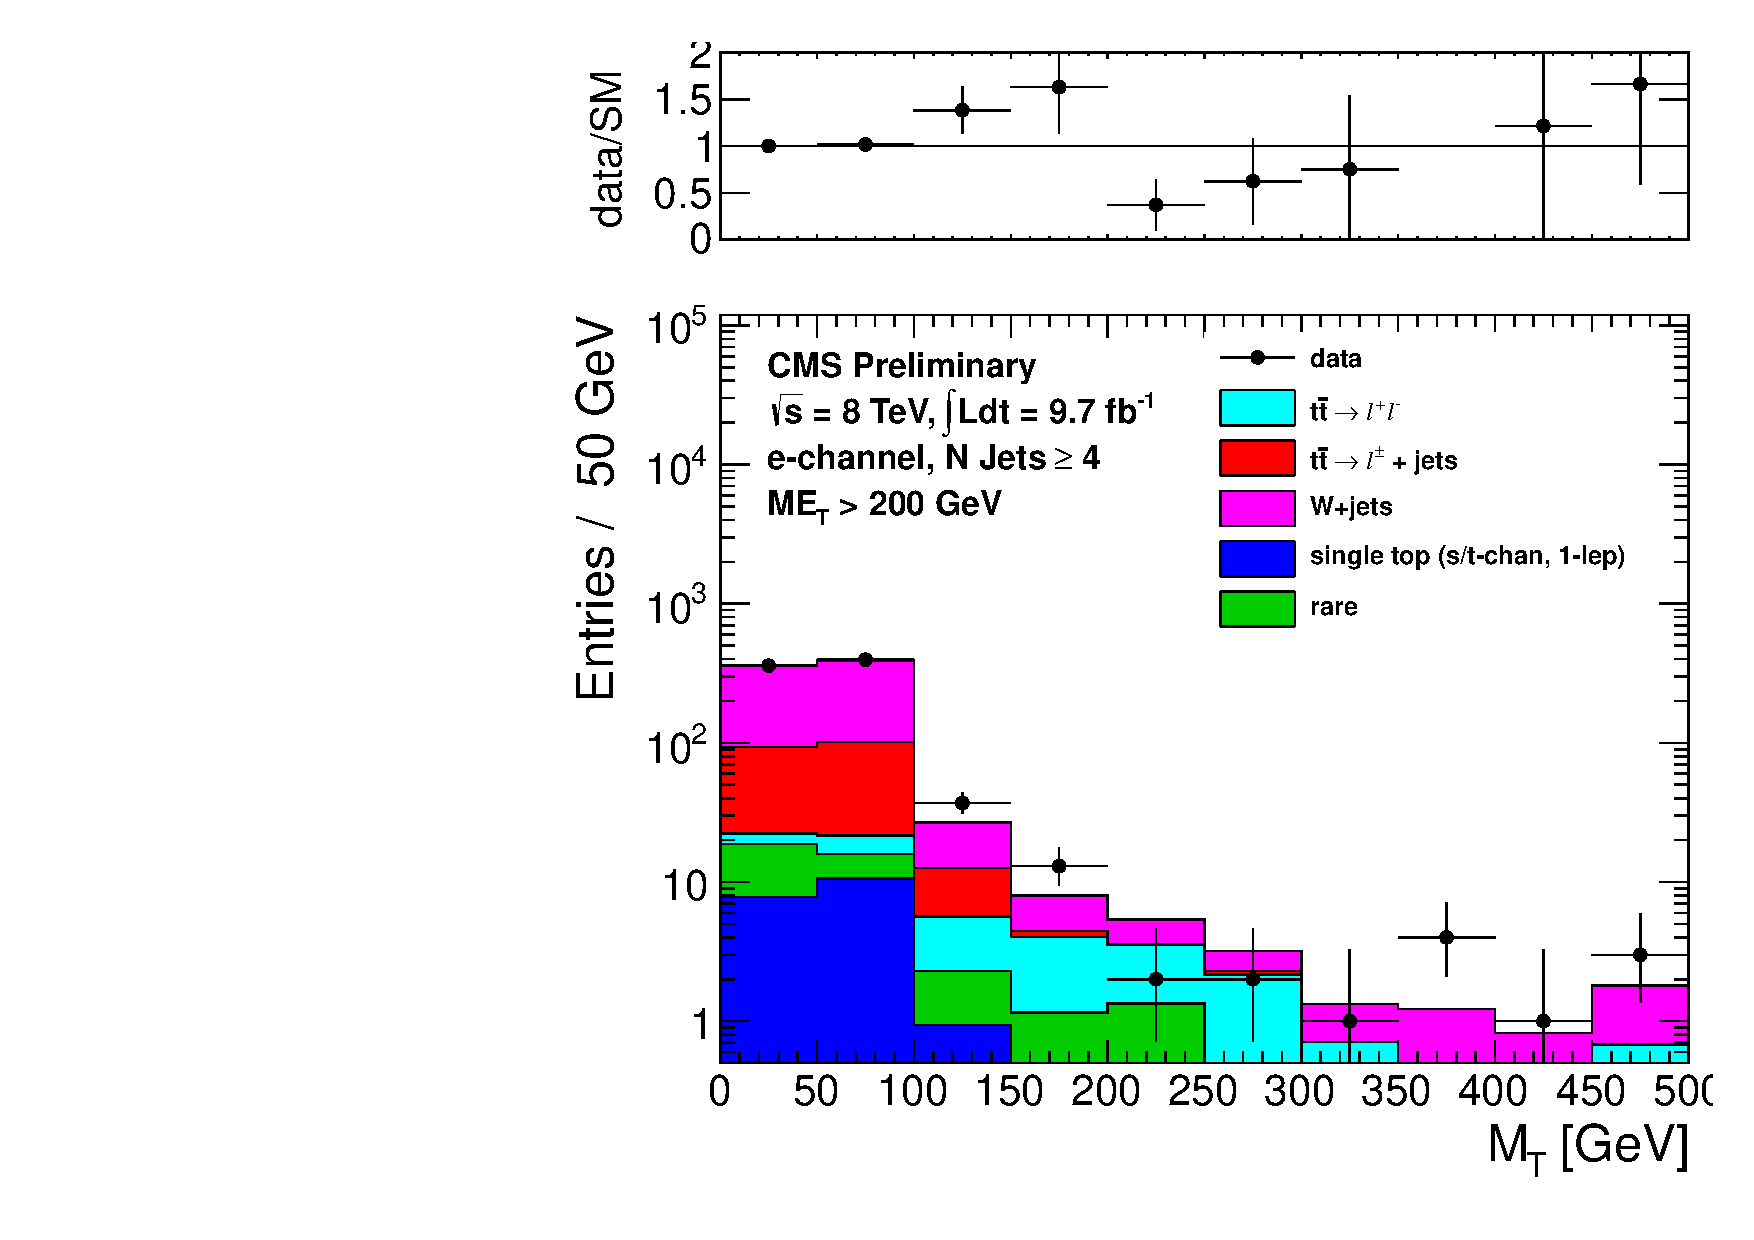
\includegraphics[width=0.5\linewidth]{plots/CR1plots/mt_met200_leadele_nj4.pdf}
        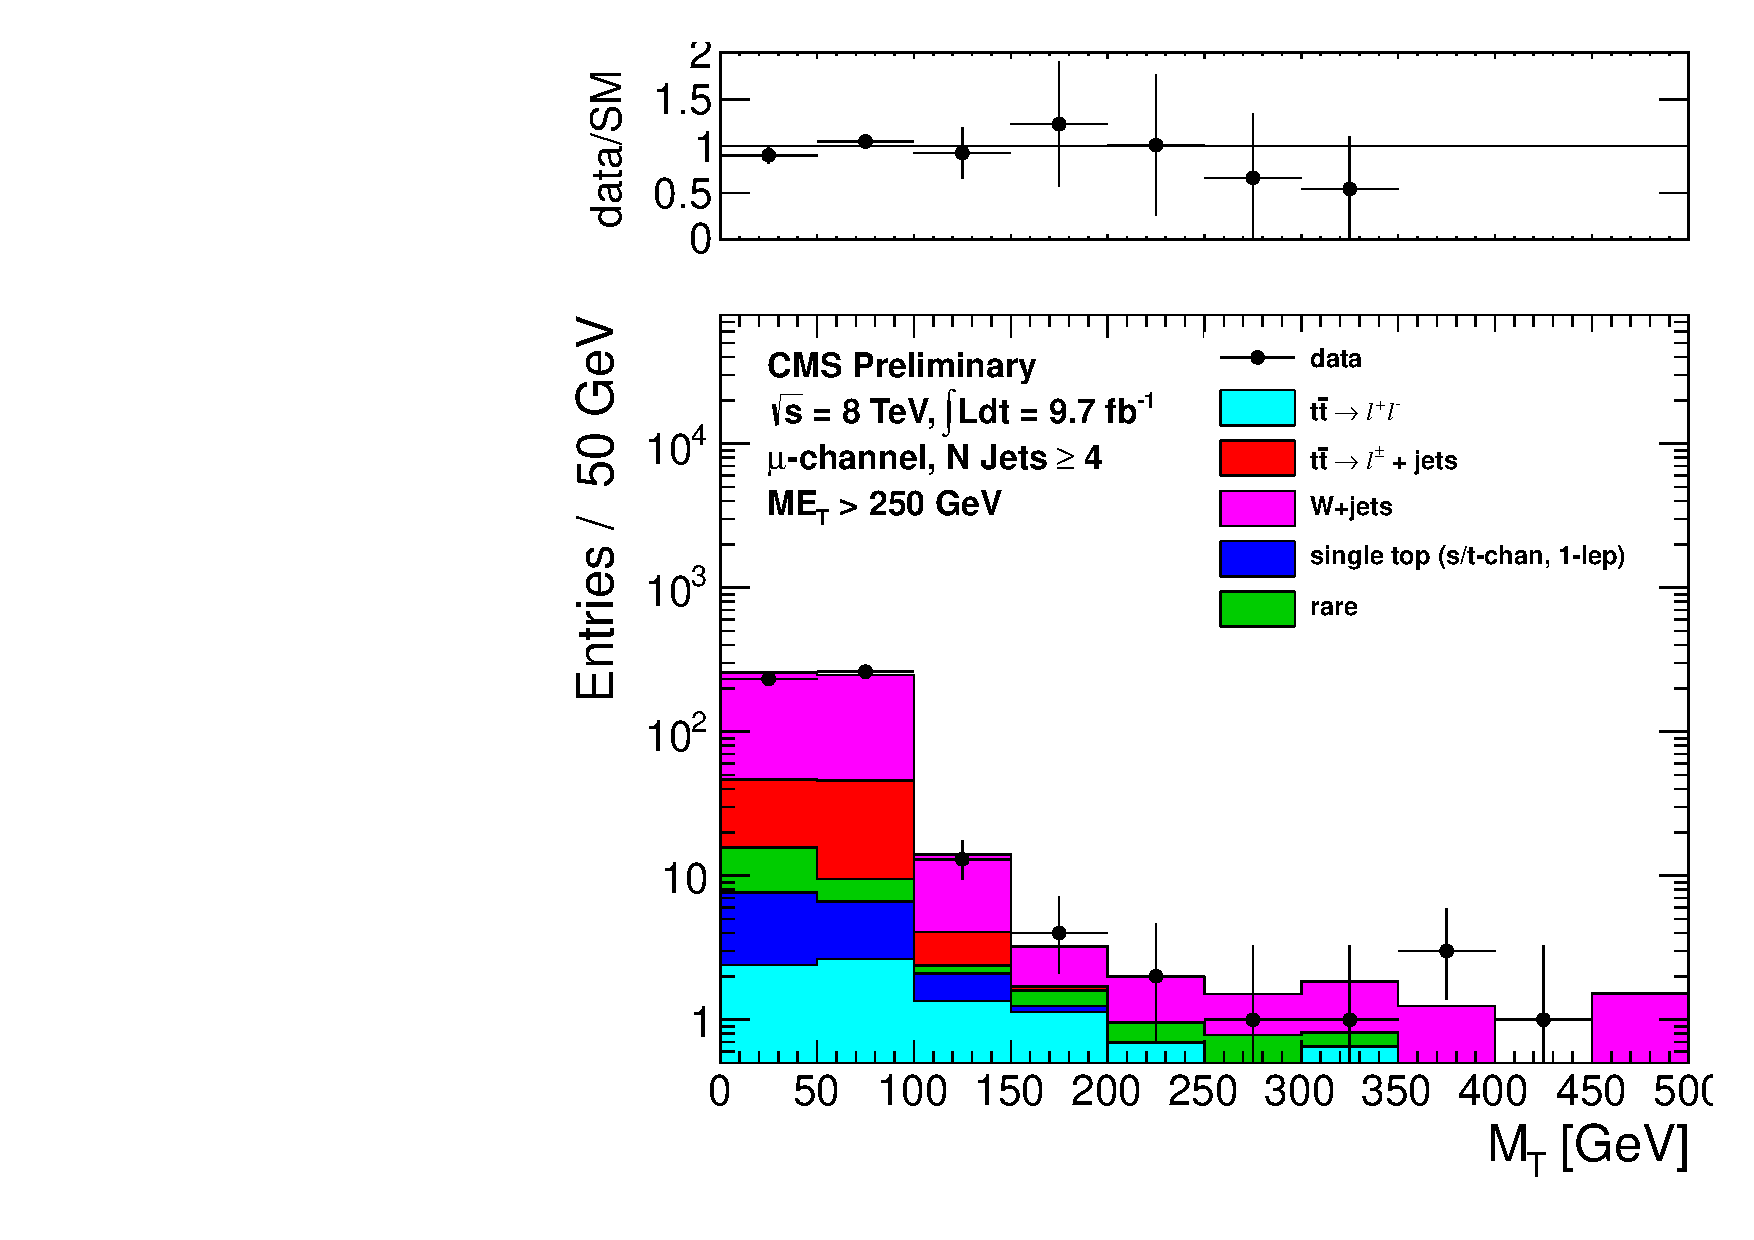
\includegraphics[width=0.5\linewidth]{plots/CR1plots/mt_met250_leadmuo_nj4.pdf}%
        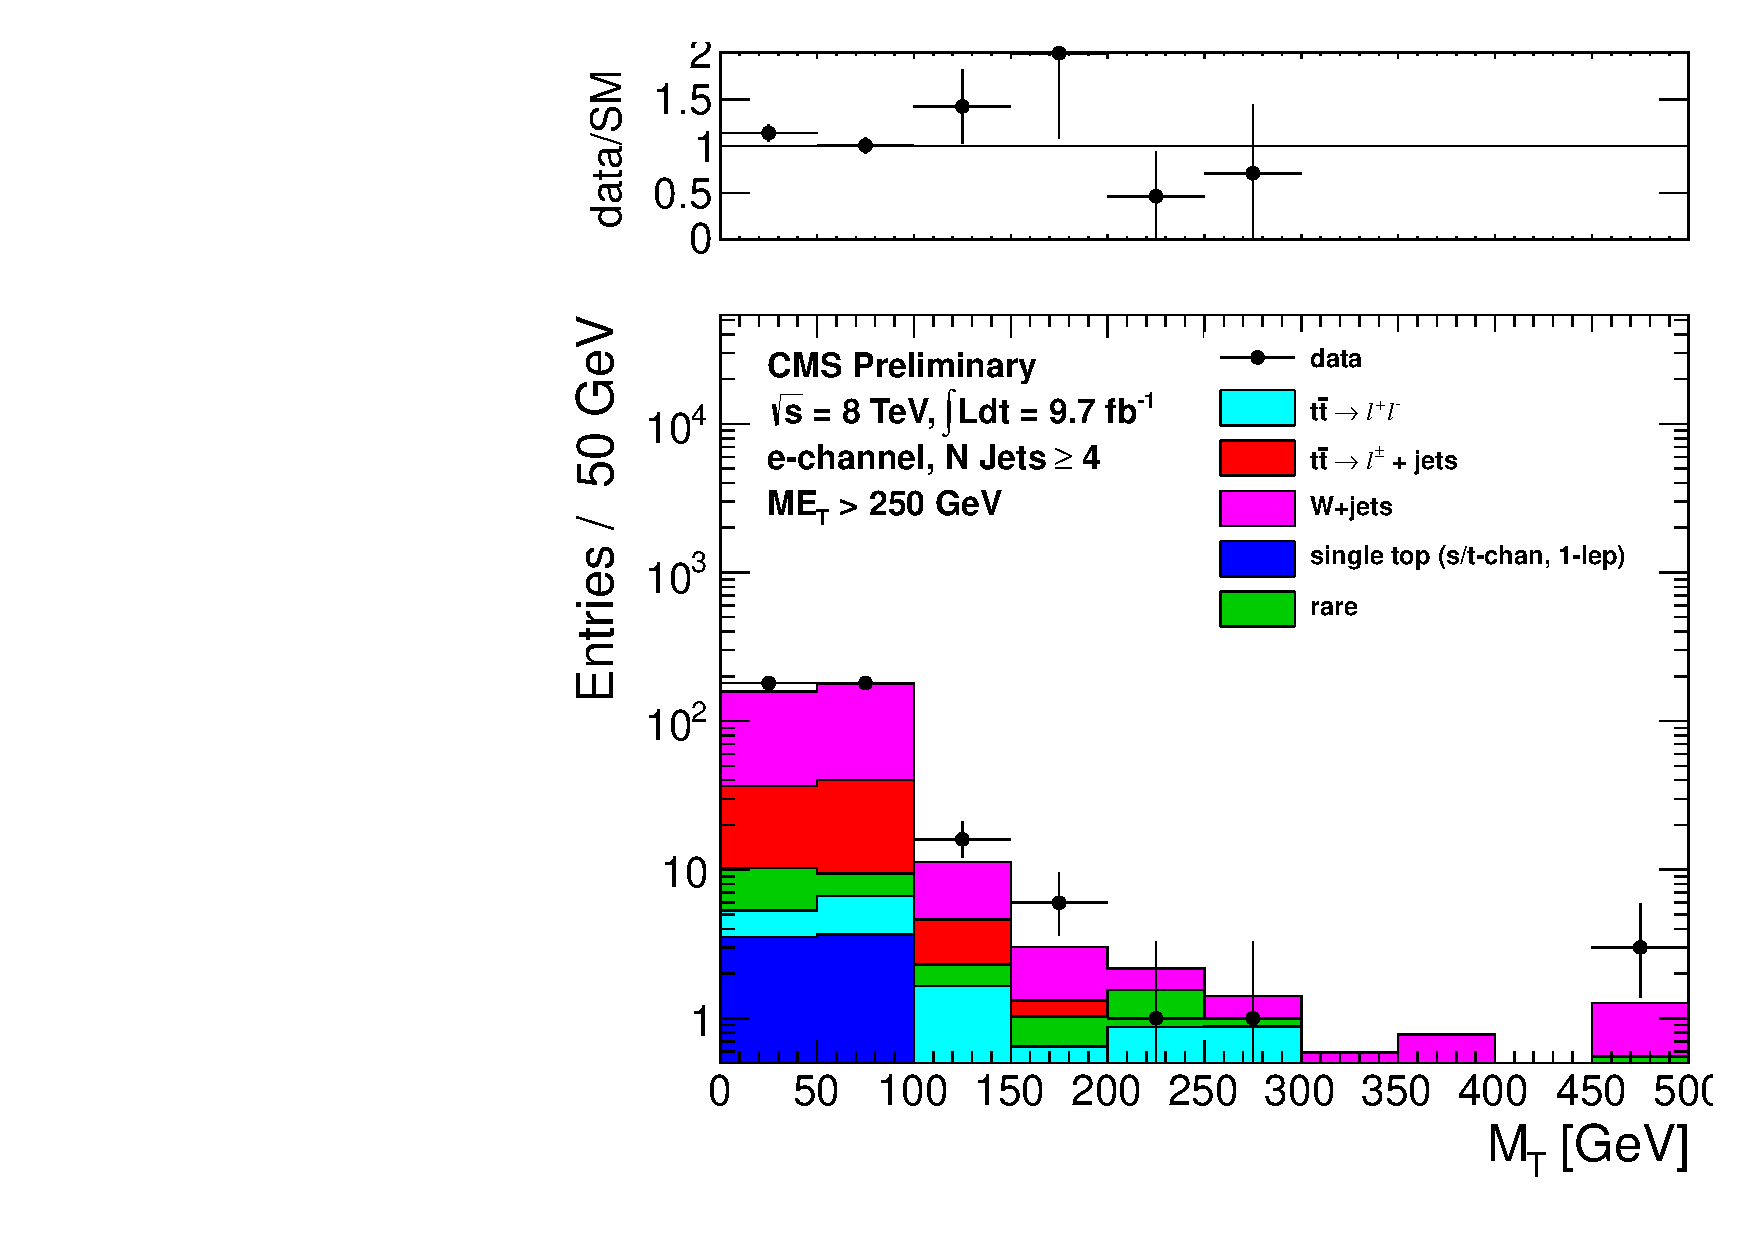
\includegraphics[width=0.5\linewidth]{plots/CR1plots/mt_met250_leadele_nj4.pdf}
    \caption{
      Comparison of the \mt\ distribution in data vs. MC for events
      with a leading muon (left) and leading electron (right)
      satisfying the requirements of CR1. The \met\ requirements used are
      150 GeV (top), 200 GeV (middle) and 250 GeV (bottom).
\label{fig:cr1mtrest} 
}  
      \end{center}
\end{figure}

\clearpage